%! Author = kaliw
%! Date = 12/10/2019

% Dense Net
\subsection{The Dense Player (aka Charmeleon)}

Our first neural net we developed, which we will refer to as Charmeleon, was created using a dense, fully connected network. We expect this net to perform much better than the random model, but worse than the upcoming convolutional model.

The network architecture we use is:
\begin{enumerate}
	\item Fully Connected 400x1
	\item ReLU
	\item Dropout (0.2)
	\item Fully Connected 300x1
	\item ReLU
	\item Fully Connected 200x1
	\item ReLU
	\item Fully Connected 125
	\item ReLU
	\item Fully Connected 75
	\item ReLU
	\item Dropout (0.1)
	\item Fully Connected 25x1
	\item ReLU
	\item Fully Connected 3x1
	\item Softmax
\end{enumerate}
This model takes a flattened game board as input as x, and the array [win, loss, draw] as y. It then evaluates the board states, learning whether a specific board state corresponding to either a win, loss, or draw. A bit of trial and error landed us on this specific architecture. Against the random model, it performed quite well, raising the win percentage from 60\% to 90\%. The full results of the models can be seen below in Table 1. 

For this model, we used an Adam optimizer with a learning rate of 0.0001, $\beta_1$ of 0.9 and $\beta_2$ of 0.999. Below you can see how results of the training runs:

\begin{figure}[h!]
	\centering
	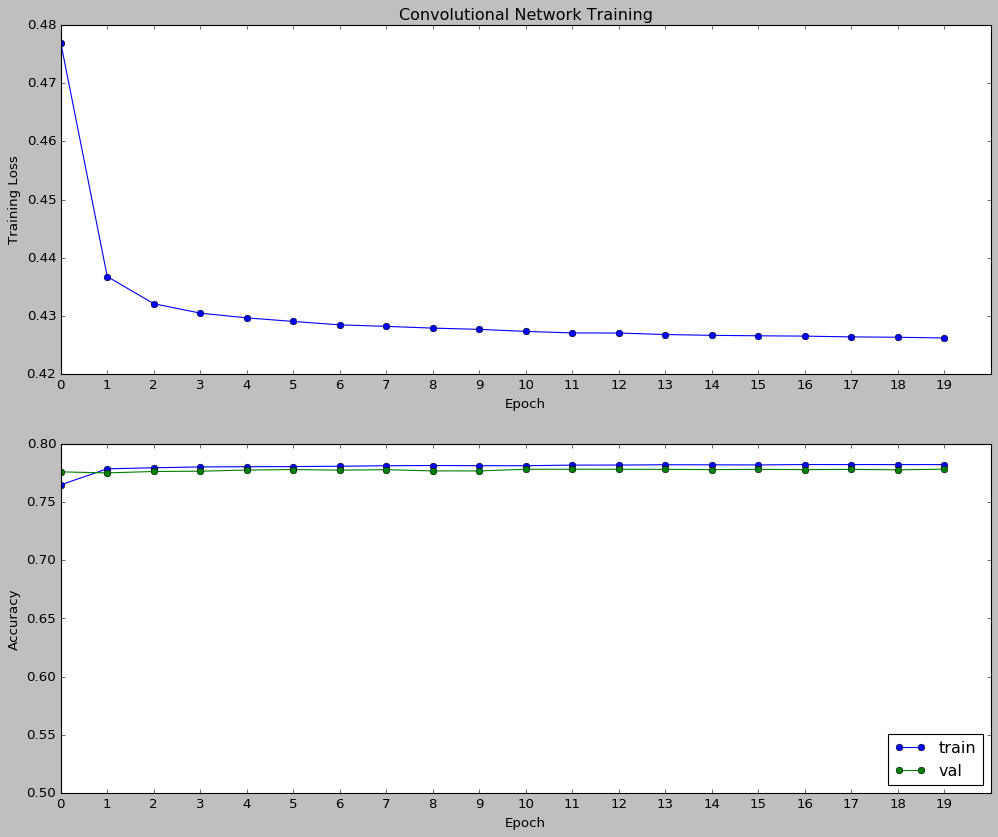
\includegraphics[width=10cm, height=7cm]{convolutional-net-training.png}
	\caption{Top: Training loss over 20 epochs. Bottom: Training accuracy against validation accuracy over 20 epochs}
	\label{fig:conv_net}
\end{figure}
